\section{Methodology}
\begin{figure}[t]\centering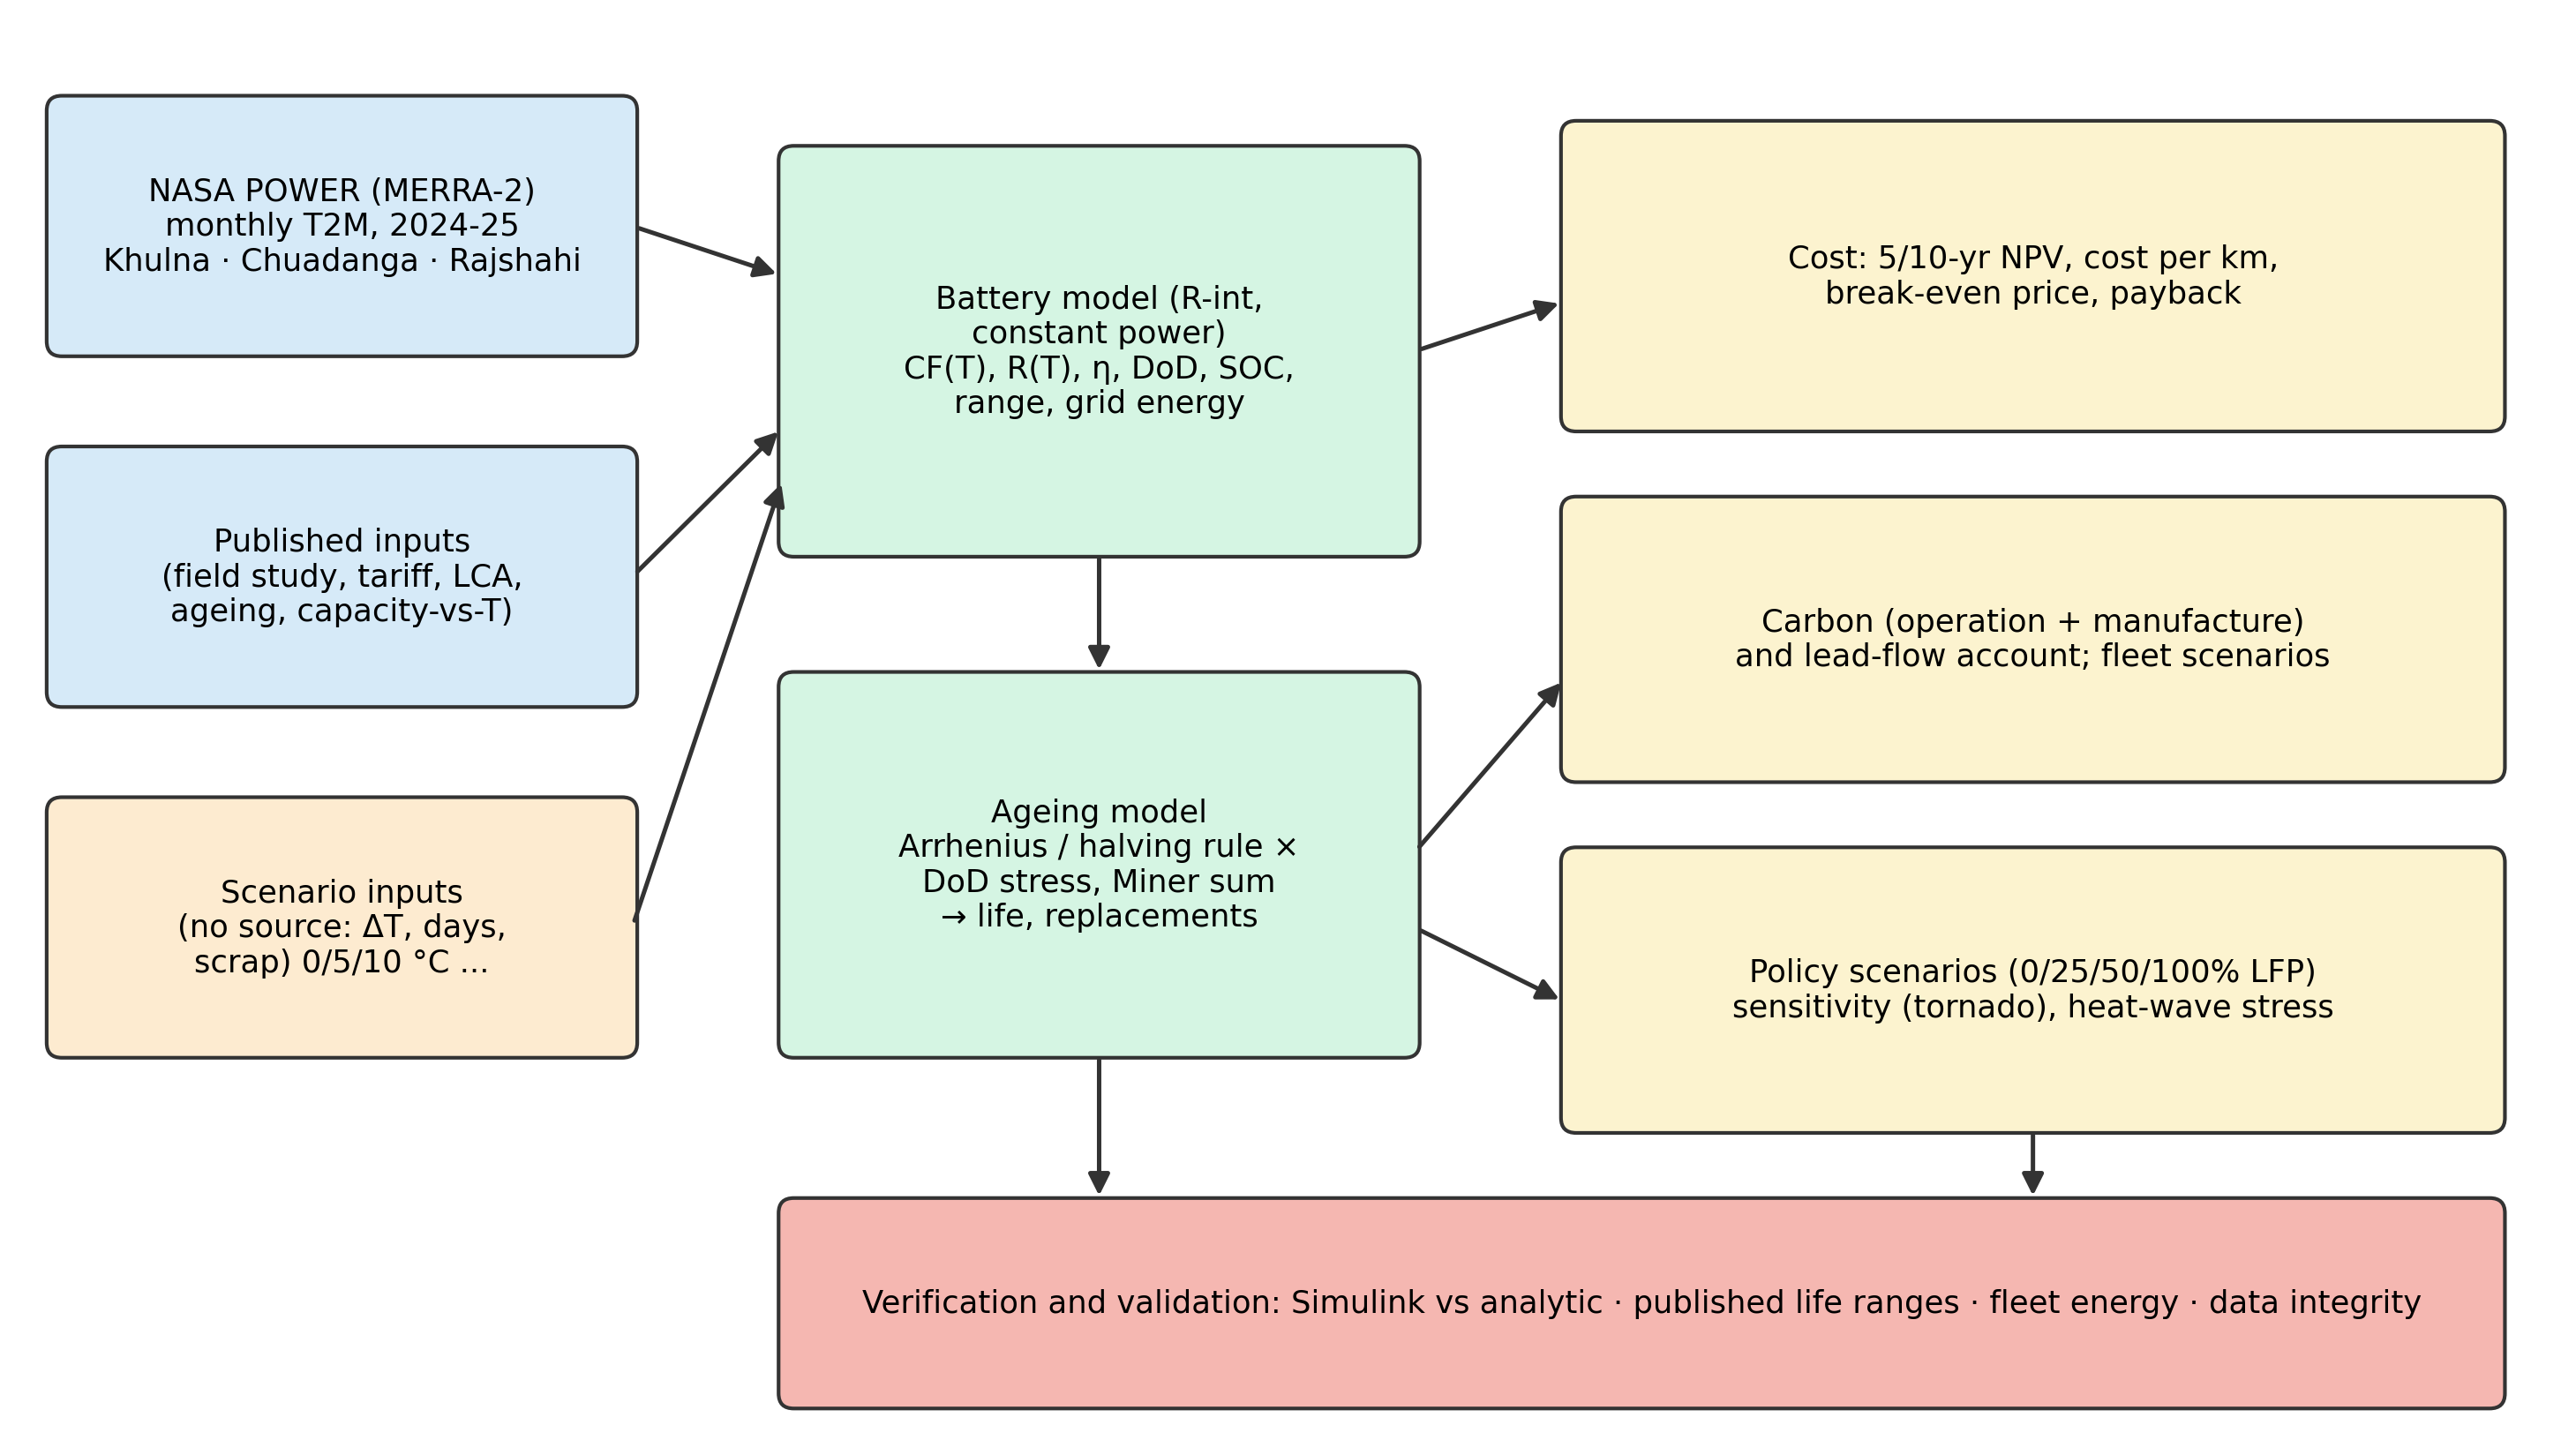
\includegraphics[width=\textwidth]{fig_method.png}\caption{Methodology: temperature and parameter inputs drive the battery and ageing models; outputs feed the cost, carbon, lead and policy modules; verification and validation close the loop.}\label{fig:method}\end{figure}
\subsection{Study design and sites}
Three south-western sites are used: Khulna (22.84$^\circ$N, 89.57$^\circ$E), Chuadanga (23.64$^\circ$N, 88.69$^\circ$E) and Rajshahi (24.38$^\circ$N, 88.60$^\circ$E) (\cref{fig:map}). Chuadanga was selected because a 42$^\circ$C day was reported there in May 2025 \citep{heat2025}, giving a heat-stress case; note that in the NASA monthly means its annual mean (\TannChuadangaBtwofive$^\circ$C in 2025) is not higher than Khulna's (\TannKhulnaBtwofive$^\circ$C), so its selection rests on peak heat, not on the mean. Khulna is also one of the two districts of the field study that supplies the duty-cycle inputs \citep{chowdhury2026}. Three chemistries are compared: lead-acid (LA), LFP and NMC. No operator survey was possible, so every duty-cycle input is taken from published sources or run as a scenario (\cref{tab:params}).
\begin{figure}[t]\centering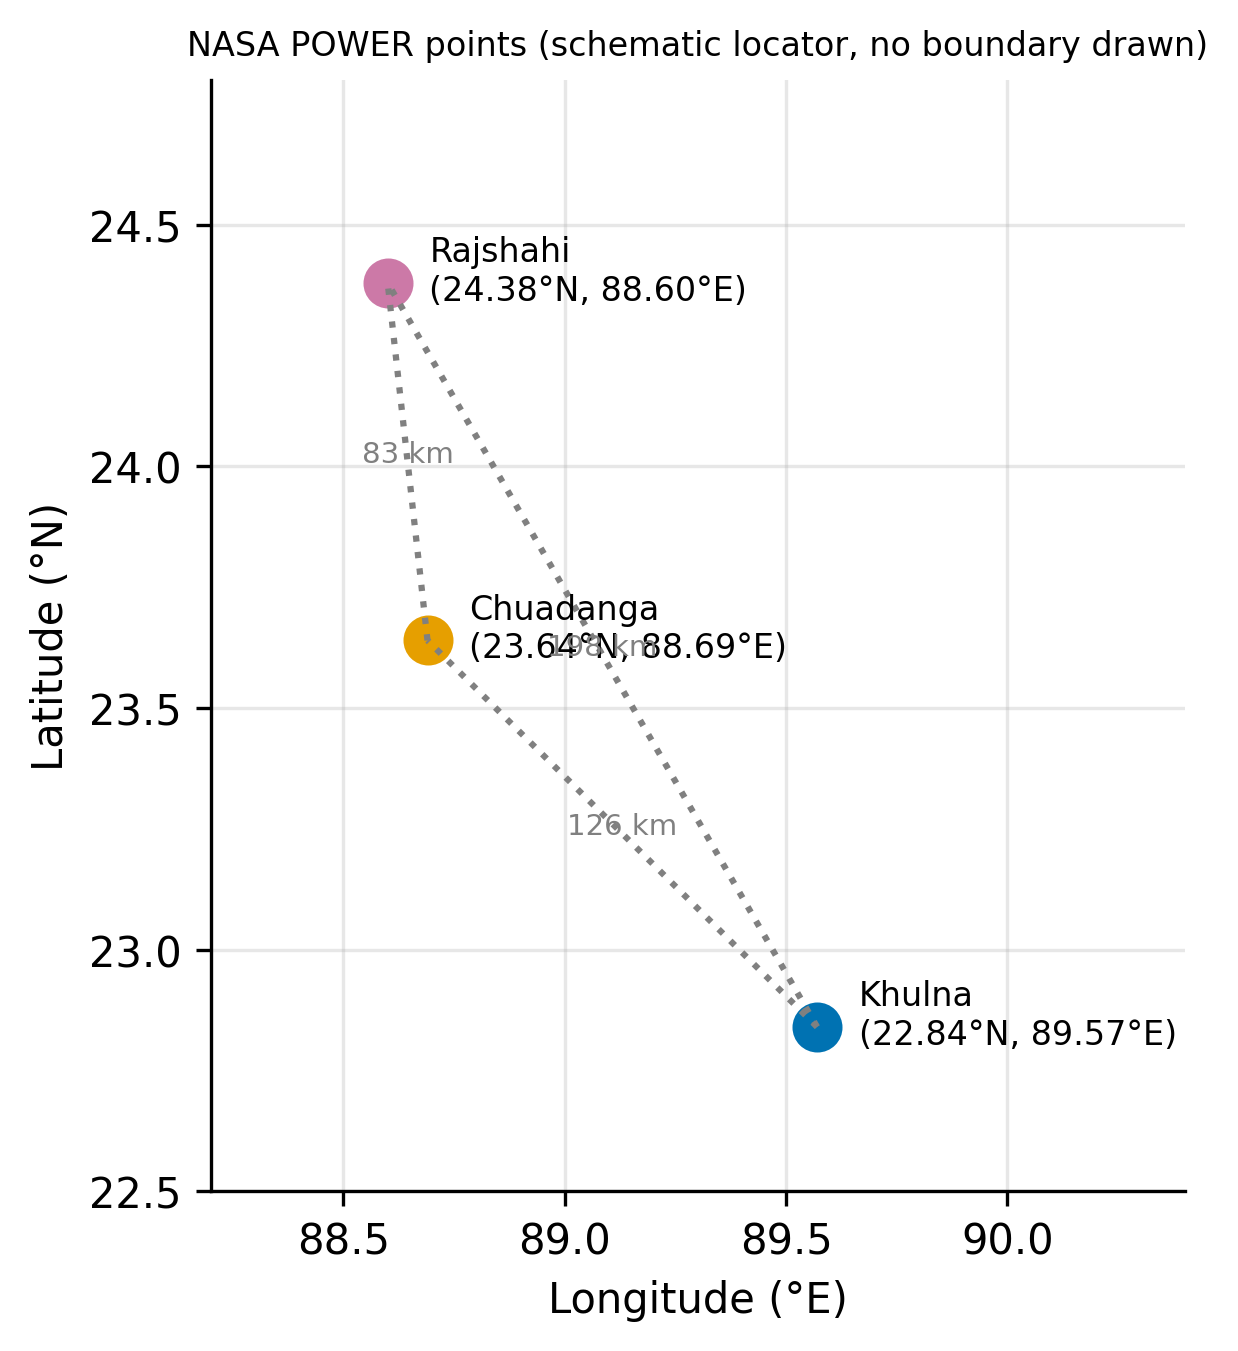
\includegraphics[width=.5\textwidth]{fig_map.png}\caption{NASA POWER grid points used (schematic locator; distances are great-circle).}\label{fig:map}\end{figure}

\subsection{Temperature data}
Monthly mean 2\,m air temperature (T2M, MERRA-2 \citep{gelaro2017}) for January 2024 to December 2025 was downloaded from NASA POWER \citep{nasa_power}: 24 values per site, no missing (-999) entries. The native cell is $0.5^\circ\times0.625^\circ$ (about 50--70~km), so the three points lie in neighbouring cells and are expected to be similar. Battery temperature is ambient plus $\Delta T_{op}=5^\circ$C, a scenario value tested at 0 and 10$^\circ$C. Monthly means understate daily peaks (\cref{sec:limits}).

\subsection{Battery model}
Each pack is a resistive (R-int) battery with temperature-dependent capacity and resistance, discharged at constant average power $P_w=e_{km}v$. With pack voltage $V$ and round-trip efficiency $\eta_{RT}$, the 25$^\circ$C resistance is chosen so that discharge efficiency equals $\sqrt{\eta_{RT}}$ at 25$^\circ$C:
\begin{equation}
R_{25}=\frac{(1-\sqrt{\eta_{RT}})\sqrt{\eta_{RT}}\,V^{2}}{P_w},\quad
R(T)=R_{25}\exp\!\left[\frac{E_r}{R_g}\!\left(\frac1{T_K}-\frac1{298.15}\right)\right],\quad
I=\frac{V-\sqrt{V^{2}-4R(T)P_w}}{2R(T)},\quad
\eta_d=1-\frac{I\,R(T)}{V}.
\end{equation}
The capacity factor $CF(T)$ is interpolated from a table, so the available energy is $E_{cap}=V\,Ah\,CF(T)/1000$~kWh. With daily delivered energy $E_{day}=d\,e_{km}/1000$ for distance $d$:
\begin{align}
DoD&=\frac{E_{day}}{\eta_d\,E_{cap}}, & SOC_{end}&=\max(0,1-DoD),\\
E_{grid}&=\frac{E_{day}}{\eta_d^{2}\,\eta_{chg}}, & \text{Range}&=\frac{DoD_{max}\,E_{cap}\,\eta_d}{e_{km}/1000}.
\end{align}
The same equations are implemented as a Simulink model built from core blocks (\cref{fig:simulink}): constant, lookup tables, product, a function block for the constant-power current, an integrator for SOC, and a sum. It is run at 15, 25, 35 and 45$^\circ$C for all three chemistries and compared with the analytic code (\texttt{easybike\_build\_simulink.m}); the acceptance criterion is 0.5 percentage points in efficiency, 0.01 in end-of-day SOC and 2\% in range. \todo{run easybike\_build\_simulink in MATLAB and report the PASS table here}
\begin{figure}[t]\centering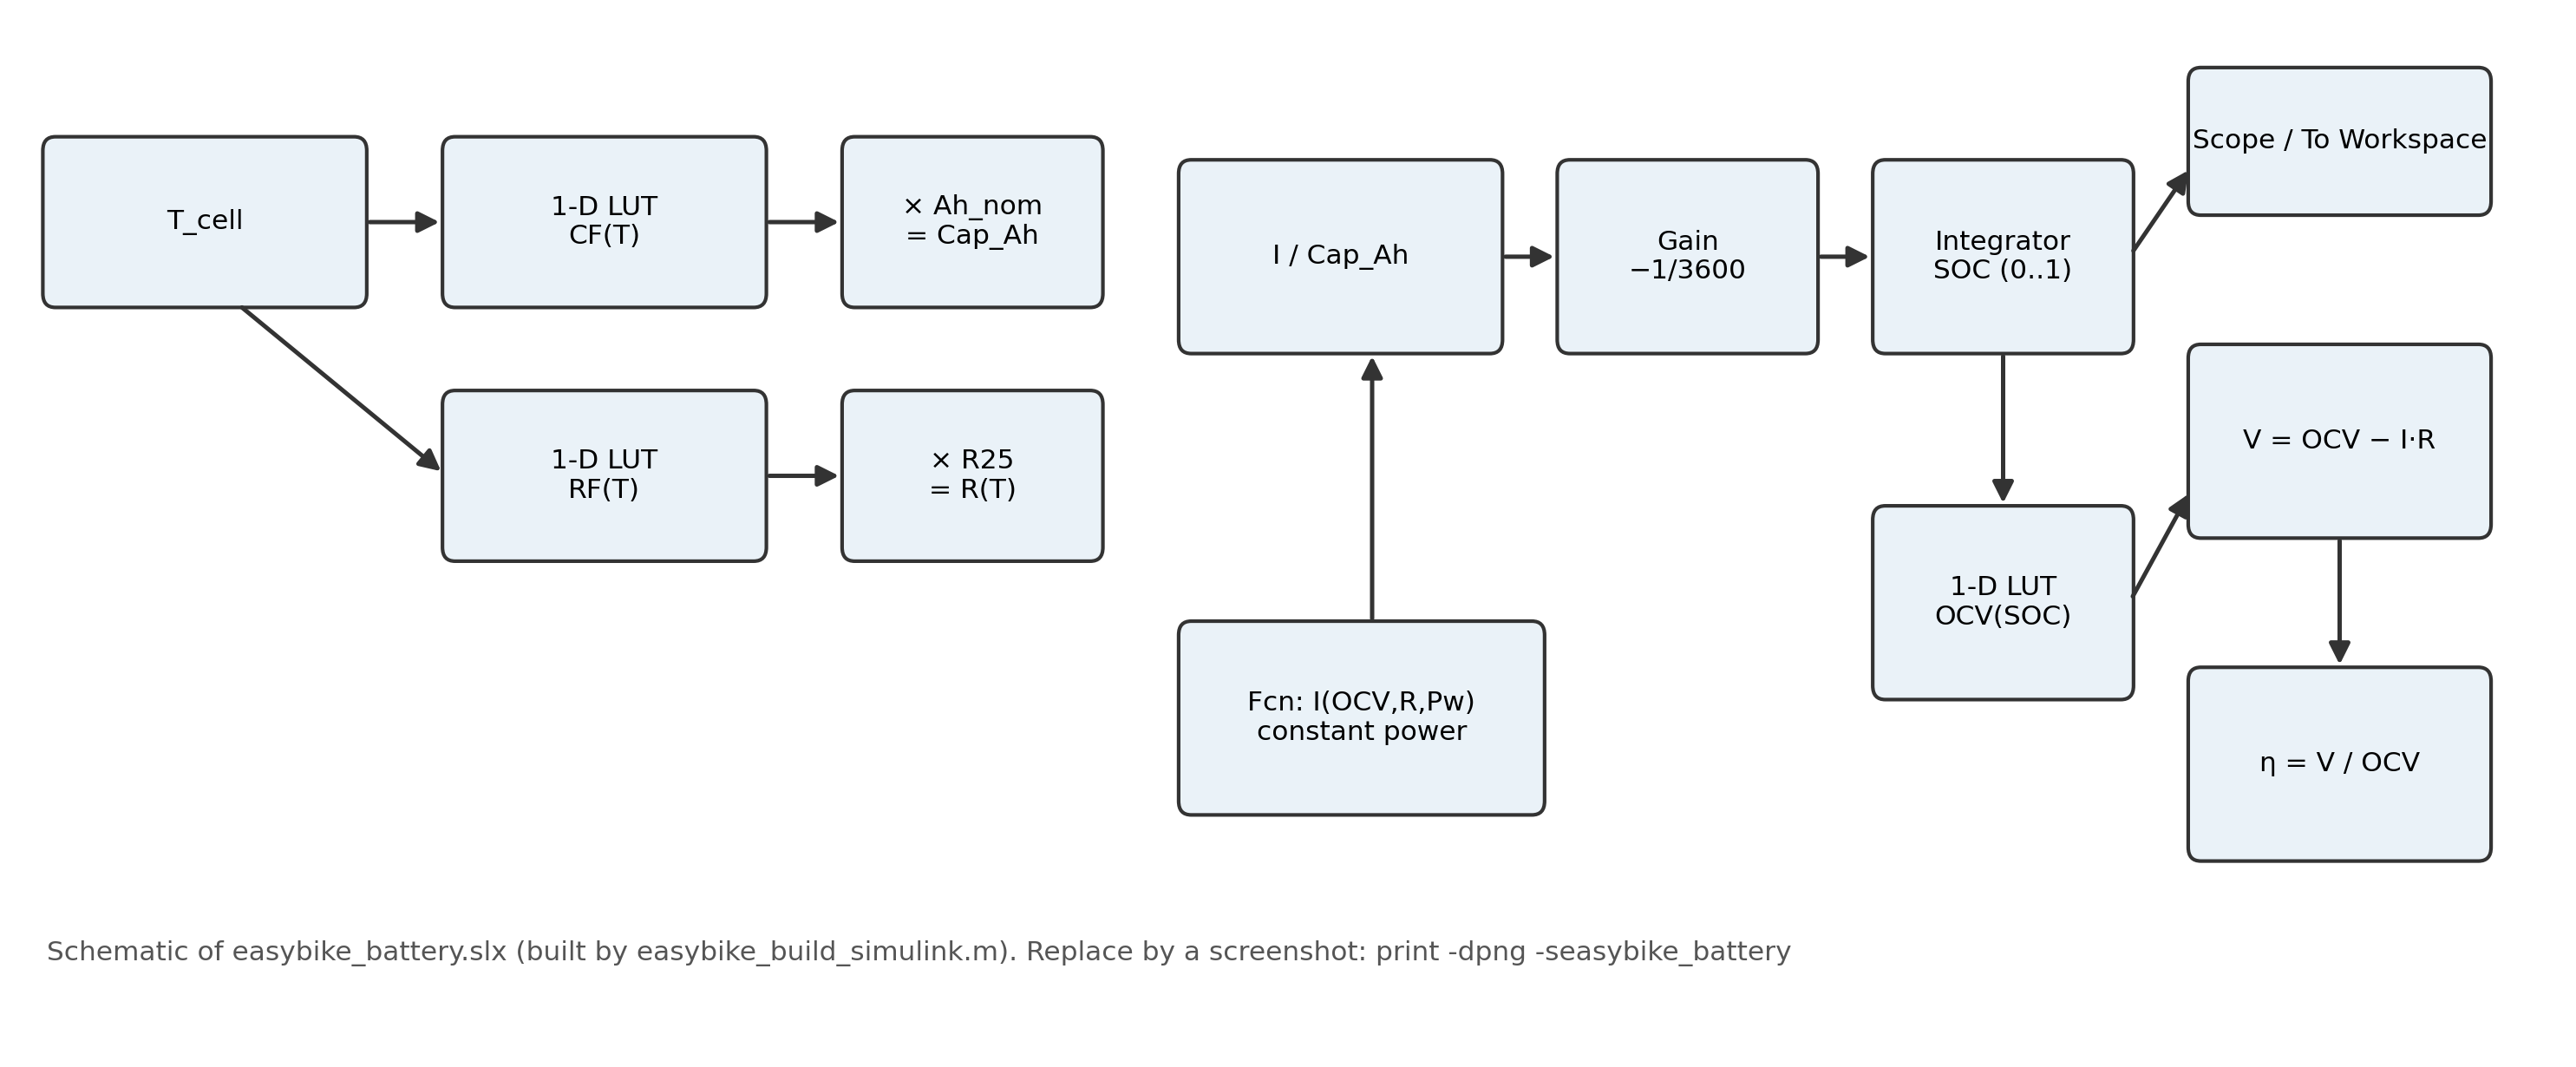
\includegraphics[width=\textwidth]{fig_simulink.png}\caption{Block structure of the Simulink model \texttt{easybike\_battery.slx} (schematic). \todo{optional: replace by a screenshot of the model}}\label{fig:simulink}\end{figure}

\subsection{Degradation and lifetime}
Cycle life falls with depth of discharge and temperature, and damage is accumulated month by month with Miner's rule \citep{miner1945}, as also done for variable-temperature VRLA service \citep{tsujikawa2009}:
\begin{equation}
N_{eff,m}=N_{80}\left(\frac{0.8}{\max(DoD_m,0.05)}\right)^{k} f_T(T_m),\qquad
D=n_{cyc}\sum_m \frac{w_m}{N_{eff,m}},\qquad
L=\frac{1}{D\,d_{op}}\ \text{(years)},
\end{equation}
where $w_m$ is the day-weighted share of month $m$, $d_{op}=300$ operating days per year and $n_{cyc}=1$. For lithium, $f_T=\min\{1,\exp[\tfrac{E_a}{R_g}(\tfrac1{T_K}-\tfrac1{298.15})]\}$ with $E_a=37.3$~kJ/mol (LFP, \citep{yagci2026}) and 10.3~kJ/mol (NMC, derived from \citep{jalkanen2015}); for lead-acid $f_T=\min\{1,2^{-(T-25)/8}\}$ \citep{bu806a}. The cap at 1 gives no life credit below 25$^\circ$C. Calendar ageing is not modelled, so life is cycle-limited (\cref{sec:limits}).

\subsection{Total cost of ownership}
The 5- and 10-year net present cost with discount rate $r$ is
\begin{equation}
TCO_H=C_0+\sum_{j=1}^{K}\frac{C_0(1-s)}{(1+r)^{jL}}-\frac{C_0\,\rho_H}{(1+r)^{H}}+\sum_{t=1}^{H}\frac{E_{grid}\,d_{op}\,\tau + m\,C_0}{(1+r)^t},
\end{equation}
with $C_0$ the pack price, $K=\lfloor H/L\rfloor$ replacements, $s$ the scrap fraction, $\rho_H$ the residual life fraction at horizon $H$, $\tau$ the tariff and $m$ the maintenance fraction. Cost per km is $TCO_{10}$ divided by the discounted distance. The cost is battery-related only (vehicle and driver costs are excluded).

\subsection{Carbon, lead and policy}
Annual emissions per bike are $E_{CO_2}=E_{grid}\,d_{op}\,EF_{grid}+\varepsilon\,Q_{nom}\,12/L_{mo}$ with $EF_{grid}=0.62$~tCO$_2$/MWh \citep{doe_gef}, $Q_{nom}$ the pack energy, $L_{mo}$ the life in months and $\varepsilon=40$, 50, 78.4~kg\,CO$_2$e/kWh (LA, LFP, NMC; \citep{jasper2025,paul2024}). The NMC value is cell-level and the factors come from European studies; Li packs are imported, so LFP is tested up to 110~kg\,CO$_2$e/kWh. A second estimate scales the CLEAN fleet electricity by the modelled LFP-to-LA grid-energy ratio. Informal-smelting emissions have no verified factor and are excluded, which biases the lead-acid footprint downward. Lead cycled per year is $M_{Pb}=N\,m_{Pb}\,12/L_{mo}$ with $m_{Pb}=60$, 90, 125~kg per pack: a mass flow, not an emission or a dose. Policy scenarios move a share $\phi=0$, 25, 50, 100\% of a 1.4~M fleet from LA to LFP; outputs scale linearly.

\subsection{Validation and sensitivity}
Five checks are made: V1 data integrity; V2 energy use against published values (a 110~km-per-charge benchmark of five 120~Ah batteries \citep{techno2016} and 71.4--88~Wh/km \citep{peakdemand}); V3 modelled life against reported ranges (8--12 months for lead-acid \citep{fe2024}; 60--84 and 36--48 months for LFP and NMC from the data file); V4 grid energy against the 8--9~kWh per charge of the field study \citep{chowdhury2026} (used for calibration, so not independent) and against the CLEAN fleet figure (independent); V5 Simulink against the analytic model. One-at-a-time sensitivity (11 inputs, \cref{fig:tornado}) and scenario runs for battery temperature, distance, scrap value and tariff address inputs without a published source.
